\documentclass[12pt,a4paper]{article}

% ─── Page Layout ───────────────────────────────────────────────────────────────
\usepackage[a4paper, margin=0.8in, headheight=14pt]{geometry}

% ─── Fonts (XeLaTeX) ───────────────────────────────────────────────────────────
\usepackage{fontspec}
\usepackage{unicode-math}
\setmainfont{TeX Gyre Pagella}
\setmonofont[Scale=0.88]{TeX Gyre Cursor}
\setmathfont{Latin Modern Math}

% ─── Packages ──────────────────────────────────────────────────────────────────
\usepackage{xcolor}
\usepackage{colortbl}
\usepackage{titlesec}
\usepackage{enumitem}
\usepackage{tabularx}
\usepackage{booktabs}
\usepackage{array}
\usepackage{amsmath}
\usepackage{tikz}
\usetikzlibrary{shapes.geometric, arrows.meta, positioning, calc, fit, decorations.pathreplacing}
\usepackage{tcolorbox}
\tcbuselibrary{skins, breakable}
\usepackage{hyperref}
\usepackage{fancyhdr}
\usepackage{graphicx}
\usepackage{microtype}
\hyphenpenalty=10000
\exhyphenpenalty=10000
\sloppy
\usepackage{caption}
\usepackage{setspace}
\usepackage{multirow}
\usepackage{tocloft}

% ─── Q&A helper ────────────────────────────────────────────────────────────────
\newcommand{\Q}[1]{\textbf{#1}\par\noindent\ignorespaces}

% ─── Colour Palette ────────────────────────────────────────────────────────────
\definecolor{myred}{RGB}{196,30,58}
\definecolor{mydark}{RGB}{30,30,50}
\definecolor{mygreen}{RGB}{14,120,80}
\definecolor{myteal}{RGB}{0,130,140}
\definecolor{myamber}{RGB}{180,100,0}
\definecolor{mypurple}{RGB}{100,30,160}
\definecolor{mygray}{RGB}{246,247,249}
\definecolor{mgframe}{RGB}{180,185,200}
\definecolor{watermark}{RGB}{145,150,170}
\definecolor{hdrred}{RGB}{250,232,235}
\definecolor{hdrgreen}{RGB}{220,244,233}
\definecolor{hdrteal}{RGB}{220,242,244}
\definecolor{hdramber}{RGB}{253,242,215}
\definecolor{hdrpurple}{RGB}{238,228,255}
\definecolor{hdrgray}{RGB}{238,240,245}
\definecolor{rowalt}{RGB}{250,251,253}

% ─── Section Formatting ────────────────────────────────────────────────────────
\titleformat{\section}
  {\large\bfseries\color{myred}}{\thesection.}{0.5em}{}
  [\vspace{1pt}{\color{myred}\rule{\linewidth}{0.8pt}}]
\titleformat{\subsection}
  {\normalsize\bfseries\color{myteal}}{\thesubsection}{0.5em}{}
\titlespacing*{\section}{0pt}{18pt}{7pt}
\titlespacing*{\subsection}{0pt}{11pt}{4pt}

% ─── Paragraph ─────────────────────────────────────────────────────────────────
\setlength{\parindent}{0pt}
\setlength{\parskip}{4pt}

% ─── TOC Styling ───────────────────────────────────────────────────────────────
\renewcommand{\cfttoctitlefont}{\large\bfseries\color{myred}}
\renewcommand{\cftaftertoctitle}{\par\noindent{\color{myred}\rule{\linewidth}{0.8pt}}}
\setlength{\cftbeforetoctitleskip}{0pt}
\setlength{\cftaftertoctitleskip}{6pt}
\renewcommand{\cftsecfont}{\normalsize\bfseries\color{mydark}}
\renewcommand{\cftsecpagefont}{\normalsize\bfseries\color{mydark}}
\renewcommand{\cftsecleader}{\cftdotfill{\cftdotsep}}
\setlength{\cftbeforesecskip}{7pt}
\renewcommand{\cftsubsecfont}{\small\color{mydark}}
\renewcommand{\cftsubsecpagefont}{\small\color{mydark}}
\setlength{\cftbeforesubsecskip}{3pt}
\setlength{\cftsubsecindent}{1.4em}

% ─── Table helpers ─────────────────────────────────────────────────────────────
\renewcommand{\arraystretch}{1.45}
\setlength{\tabcolsep}{6pt}
\arrayrulecolor{mydark}
\newcolumntype{B}[1]{>{\small\bfseries\raggedright\arraybackslash}m{#1}}
\newcolumntype{Y}{>{\small\raggedright\arraybackslash}X}
\renewcommand{\tabularxcolumn}[1]{m{#1}}

% ─── Header / Footer ───────────────────────────────────────────────────────────
\pagestyle{fancy}
\fancyhf{}
\fancyhead[L]{\small\color{myred}\textbf{HS-HU701}\;\color{mydark}--- Principles of Management}
\fancyhead[R]{\small\color{myteal}\textbf{Module 1 Notes}}
\fancyfoot[C]{\small\color{mydark}\thepage}
\fancyfoot[R]{\small\color{watermark}\textit{\copyright\ Biraj}}
\renewcommand{\headrulewidth}{0.5pt}
\renewcommand{\footrulewidth}{0.3pt}

% ─── Hyperref ──────────────────────────────────────────────────────────────────
\hypersetup{
  colorlinks=true, linkcolor=myteal, urlcolor=myteal,
  pdfauthor={Biraj Sarkar},
  pdftitle={HS-HU701 --- Module 1 Notes}
}

% ─── tcolorbox styles ──────────────────────────────────────────────────────────
\tcbset{
  tikzbox/.style={
    colback=mygray, colframe=mgframe, boxrule=0.6pt, arc=4pt,
    left=8pt, right=8pt, top=6pt, bottom=6pt,
    colbacktitle=mgframe, coltitle=mydark,
    fonttitle=\small\bfseries
  },
  defbox/.style={
    colback=hdrgreen, colframe=mygreen, boxrule=0.8pt, arc=4pt,
    left=9pt, right=9pt, top=6pt, bottom=6pt,
    colbacktitle=mygreen, coltitle=white,
    fonttitle=\small\bfseries
  },
  formulabox/.style={
    colback=hdrteal, colframe=myteal, boxrule=0.8pt, arc=4pt,
    left=9pt, right=9pt, top=7pt, bottom=7pt,
    colbacktitle=myteal, coltitle=white,
    fonttitle=\small\bfseries
  },
  examplebox/.style={
    colback=hdramber, colframe=myamber, boxrule=0.8pt, arc=4pt,
    left=9pt, right=9pt, top=6pt, bottom=6pt,
    colbacktitle=myamber, coltitle=white,
    fonttitle=\small\bfseries
  },
  masonbox/.style={
    colback=hdrpurple, colframe=mypurple, boxrule=0.8pt, arc=4pt,
    left=9pt, right=9pt, top=6pt, bottom=6pt,
    colbacktitle=mypurple, coltitle=white,
    fonttitle=\small\bfseries
  },
  exambox/.style={
    colback=hdrpurple, colframe=mypurple, boxrule=1pt, arc=5pt,
    left=10pt, right=10pt, top=8pt, bottom=8pt,
    colbacktitle=mypurple, coltitle=white,
    fonttitle=\bfseries,
    breakable, title after break={\textbf{Frequently Asked / Viva Questions (contd.)}}}
}
\tcbset{breakable}

% ─── TikZ styles ───────────────────────────────────────────────────────────────
\tikzset{
  block/.style={rectangle, draw=myteal, fill=hdrteal,
    text width=2.4cm, align=center, minimum height=0.95cm,
    font=\small, rounded corners=3pt, line width=0.7pt},
  redblock/.style={rectangle, draw=myred, fill=hdrred,
    text width=2.4cm, align=center, minimum height=0.95cm,
    font=\small, rounded corners=3pt, line width=0.7pt},
  netnode/.style={rectangle, draw=myteal, fill=hdrteal,
    text width=1.5cm, align=center, minimum height=0.8cm,
    font=\small, rounded corners=3pt, line width=0.7pt},
  sumjunc/.style={circle, draw=myamber, fill=hdramber,
    minimum size=0.62cm, font=\small, line width=0.8pt},
  snode/.style={circle, draw=mypurple, fill=hdrpurple,
    minimum size=0.55cm, font=\footnotesize, line width=0.7pt},
  arrow/.style={-Stealth, thick, color=mydark},
  redarrow/.style={-Stealth, thick, color=myred},
  line/.style={thick, color=mydark}
}

% ═══════════════════════════════════════════════════════════════════════════════
\begin{document}
% ═══════════════════════════════════════════════════════════════════════════════

\begin{center}
  {\LARGE\bfseries\color{myred} HS-HU701 --- Principles of Management}\\[5pt]
  {\normalsize\color{mydark} Semester VII \quad$\bullet$\quad 2L:0T:0P \quad$\bullet$\quad 2 Credits}\\[3pt]
  {\normalsize\color{myteal}\textbf{Module 1 Exam Notes}}\\[3pt]
  {\small\color{mydark} CGEC \;$|$\; B.Tech ECE (2023--27) \;$|$\; \textit{Biraj Sarkar}}
\end{center}
\vspace{2pt}
\noindent{\color{myred}\rule{\linewidth}{1.5pt}}
\vspace{2pt}

\hypersetup{linkcolor=mydark}
\tableofcontents
\hypersetup{linkcolor=myteal}
\newpage

% ===============================================================================
\section{Basic Concepts of Management}
% ===============================================================================

\begin{tcolorbox}[defbox, title={\textbf{Definition of Management}}]
\textbf{Management} is the process of planning, organising, leading, and controlling the efforts of organisational members and using all other organisational resources to achieve stated organisational goals efficiently and effectively.
\par\vspace{3pt}
\textbf{Efficiency} means doing things right (optimal resource utilisation). \textbf{Effectiveness} means doing the right things (achieving goals).
\end{tcolorbox}

\subsection{Essence of Management}
The essence of management revolves around the following core ideas:
\begin{itemize}[leftmargin=*, itemsep=3pt]
  \item \textbf{Goal-Oriented:} Management always aims at achieving specific organisational objectives.
  \item \textbf{Pervasive:} Management is universal --- it is required in all organisations (business, government, NGOs) and at all levels.
  \item \textbf{Multidimensional:} Involves managing work (tasks and activities), managing people (individuals and groups), and managing operations (processes and systems).
  \item \textbf{Continuous Process:} Management is an ongoing, never-ending process as long as the organisation exists.
  \item \textbf{Group Activity:} Management involves coordinating the efforts of a group of individuals toward a common goal.
  \item \textbf{Dynamic Function:} Management adapts to the changing internal and external environment of the organisation.
  \item \textbf{Intangible Force:} Management cannot be physically seen but its results (productivity, morale, order) are felt throughout the organisation.
\end{itemize}

\subsection{Functions of Management}
The five fundamental functions of management (as identified by Henri Fayol and later developed by others) are:

\begin{tcolorbox}[tikzbox, title={Five Functions of Management}]
\centering
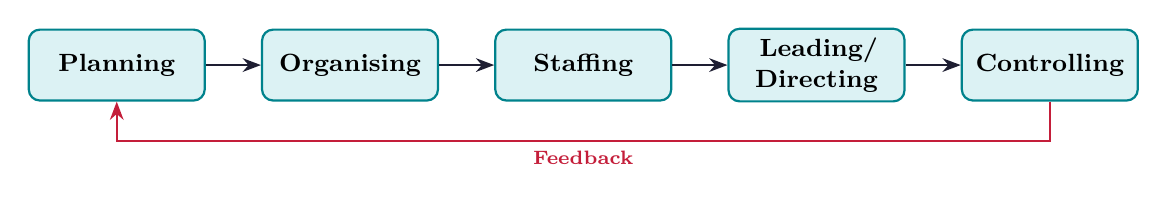
\begin{tikzpicture}[
  funcbox/.style={rectangle, draw=myteal, fill=hdrteal, text width=2.0cm,
    align=center, minimum height=0.9cm, font=\small\bfseries, rounded corners=4pt, line width=0.8pt},
  arrow/.style={-Stealth, thick, color=mydark}
]
  \node[funcbox] (plan) {Planning};
  \node[funcbox, right=0.7cm of plan] (org) {Organising};
  \node[funcbox, right=0.7cm of org] (staff) {Staffing};
  \node[funcbox, right=0.7cm of staff] (lead) {Leading/ Directing};
  \node[funcbox, right=0.7cm of lead] (ctrl) {Controlling};

  \draw[arrow] (plan) -- (org);
  \draw[arrow] (org)  -- (staff);
  \draw[arrow] (staff) -- (lead);
  \draw[arrow] (lead) -- (ctrl);
  \draw[redarrow] (ctrl.south) -- ++(0,-0.5) -| (plan.south)
    node[pos=0.25, below, font=\scriptsize\bfseries\color{myred}] {Feedback};
\end{tikzpicture}
\end{tcolorbox}

\begin{itemize}[leftmargin=*, itemsep=3pt]
  \item \textbf{Planning:} Deciding in advance what to do, how to do it, when to do it, and who is to do it. It bridges the gap between where we are and where we want to be.
  \item \textbf{Organising:} Arranging resources and tasks to achieve the plan. Involves grouping activities, assigning duties, and delegating authority.
  \item \textbf{Staffing:} Filling and keeping filled the positions in the organisation structure. Includes recruitment, selection, training, and development.
  \item \textbf{Leading/Directing:} Guiding and supervising subordinates to accomplish organisational goals. Involves communication, motivation, and leadership.
  \item \textbf{Controlling:} Measuring actual performance against planned targets and taking corrective action when necessary.
\end{itemize}

\subsection{Roles of a Manager}
Henry Mintzberg classified managerial roles into three categories based on his research on how managers actually spend their time. He identified \textbf{10 specific roles} grouped under Interpersonal, Informational, and Decisional categories. Unlike the classical view that managers only plan, organise, and control, Mintzberg showed that managerial work is varied, fragmented, and action-oriented. These roles are interlinked and a manager plays all of them simultaneously, with the emphasis shifting depending on the level and context.

\par\noindent
{\renewcommand{\arraystretch}{1.55}%
\begin{tabularx}{\linewidth}{|B{3.0cm}|Y|Y|}\hline
\multicolumn{1}{|>{\centering\arraybackslash}m{3.0cm}|}{\textbf{Category}} &
\multicolumn{1}{>{\centering\arraybackslash}Y|}{\textbf{Role}} &
\multicolumn{1}{>{\centering\arraybackslash}Y|}{\textbf{Description}} \\[4pt]
\hline
\multirow{3}{*}{\textbf{Interpersonal}} & Figurehead & Performs ceremonial duties (e.g., signing documents, representing the organisation). \\[4pt]
\hline
\cline{2-3}
& Leader & Motivates, directs, and coordinates the activities of subordinates. \\
\hline
\cline{2-3}
& Liaison & Maintains networks with outsiders and peers for information and support. \\
\hline
\multirow{3}{*}{\textbf{Informational}} & Monitor & Scans internal and external environment for information. \\[4pt]
\hline
\cline{2-3}
& Disseminator & Transmits information received from outside to members of the organisation. \\
\hline
\cline{2-3}
& Spokesperson & Transmits information to outsiders on the organisation's plans and policies. \\
\hline
\multirow{4}{*}{\textbf{Decisional}} & Entrepreneur & Initiates change; searches for new opportunities and improvement projects. \\[4pt]
\hline
\cline{2-3}
& Disturbance Handler & Takes corrective action when the organisation faces unexpected crises. \\
\hline
\cline{2-3}
& Resource Allocator & Decides who gets resources --- time, money, equipment, and manpower. \\
\hline
\cline{2-3}
& Negotiator & Represents the organisation in major negotiations with unions, suppliers, etc. \\
\hline
\end{tabularx}
}

\subsection{Levels of Management}
Management is typically divided into three hierarchical levels:

\begin{tcolorbox}[tikzbox, title={Levels of Management --- Hierarchy}]
\centering
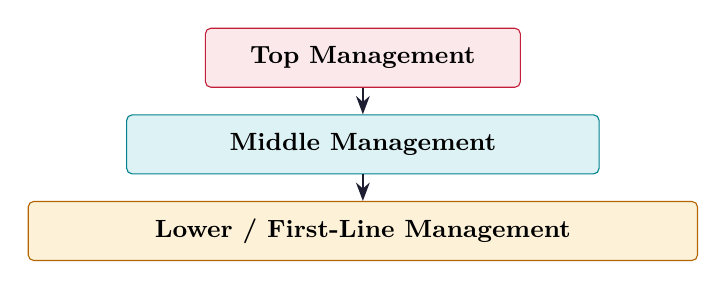
\begin{tikzpicture}
  \node[draw=myred, fill=hdrred, minimum width=4.0cm, minimum height=0.75cm,
    align=center, font=\small\bfseries, rounded corners=2pt] (top) at (0,0)
    {Top Management};
  \node[draw=myteal, fill=hdrteal, minimum width=6.0cm, minimum height=0.75cm,
    align=center, font=\small\bfseries, rounded corners=2pt] (mid) at (0,-1.1)
    {Middle Management};
  \node[draw=myamber, fill=hdramber, minimum width=8.5cm, minimum height=0.75cm,
    align=center, font=\small\bfseries, rounded corners=2pt] (low) at (0,-2.2)
    {Lower / First-Line Management};

  \draw[arrow] (top) -- (mid);
  \draw[arrow] (mid) -- (low);
\end{tikzpicture}
\end{tcolorbox}

\par\noindent
{\renewcommand{\arraystretch}{1.55}%
\begin{tabularx}{\linewidth}{|B{2.8cm}|Y|Y|}\hline
\multicolumn{1}{|>{\centering\arraybackslash}m{2.8cm}|}{\textbf{Level}} &
\multicolumn{1}{>{\centering\arraybackslash}Y|}{\textbf{Examples}} &
\multicolumn{1}{>{\centering\arraybackslash}Y|}{\textbf{Key Activities}} \\[4pt]
\hline
Top Management & CEO, MD, Board of Directors & Set overall strategy, goals, and policies; represent company externally. \\[4pt]
\hline
Middle Management & Dept. Heads, Branch Managers, General Managers & Implement top-level strategies; coordinate lower-level activities. \\[4pt]
\hline
First-Line Management & Supervisors, Foremen, Team Leaders & Direct and supervise operative employees; handle day-to-day operations. \\[4pt]
\hline
\end{tabularx}
}

% ===============================================================================
\section{Functions of Management --- Planning}
% ===============================================================================

\begin{tcolorbox}[defbox, title={\textbf{Planning --- Definition}}]
\textbf{Planning} is the primary management function that involves setting objectives and determining the best course of action to achieve them. It is forward-looking, involves decision-making, and serves as the basis for all other management functions.
\end{tcolorbox}

\subsection{Concept and Nature of Planning}
\begin{itemize}[leftmargin=*, itemsep=3pt]
  \item \textbf{Purposeful:} Planning is always directed toward the achievement of specific goals.
  \item \textbf{Primary Function:} Planning precedes all other management functions --- organising, staffing, directing, and controlling all depend on planning.
  \item \textbf{Pervasive:} All managers at all levels engage in planning, though the scope and time horizon differ.
  \item \textbf{Future-Oriented:} Planning deals with predicting future conditions and preparing for them.
  \item \textbf{Decision-Making:} Planning involves making a choice among various alternative courses of action.
  \item \textbf{Continuous Process:} Plans are constantly reviewed and revised in response to changing conditions.
  \item \textbf{Mental Exercise:} Planning requires intelligence, foresight, imagination, and sound judgment.
\end{itemize}

\subsection{Types of Plans}
\par\noindent
{\renewcommand{\arraystretch}{1.55}%
\begin{tabularx}{\linewidth}{|B{3.0cm}|Y|Y|}\hline
\multicolumn{1}{|>{\centering\arraybackslash\color{white}}m{3.0cm}|}{\textbf{Type}} &
\multicolumn{1}{>{\centering\arraybackslash\color{white}}Y|}{\textbf{Description}} &
\multicolumn{1}{>{\centering\arraybackslash\color{white}}Y|}{\textbf{Example}} \\[4pt]
\hline
Mission/Purpose & Fundamental reason for the organisation's existence. & ``Provide affordable, clean energy to all.'' \\[4pt]
\hline
Objectives/Goals & Specific, measurable targets to be achieved within a time frame. & Increase sales by 20\% in FY 2026. \\[4pt]
\hline
Strategies & Long-term, broad plans to achieve objectives in a competitive environment. & Market penetration, diversification. \\[4pt]
\hline
Policies & General guidelines that channel thinking and decision-making. & ``All employees must follow the safety code.'' \\[4pt]
\hline
Procedures & Step-by-step sequences for handling recurring activities. & Leave application procedure. \\[4pt]
\hline
Rules & Specific, definite actions or prohibitions with no discretion. & ``No smoking in office premises.'' \\[4pt]
\hline
Programmes & Complex of goals, policies, procedures, and budgets for a major action. & Employee training programme. \\[4pt]
\hline
Budgets & A plan expressed in numerical terms (usually money or units). & Annual capital expenditure budget. \\[4pt]
\hline
\end{tabularx}
}

\subsection{Management by Objectives (MBO)}

\begin{tcolorbox}[defbox, title={\textbf{MBO --- Definition}}]
\textbf{Management by Objectives (MBO)}, developed by Peter Drucker (1954), is a management philosophy in which superiors and subordinates jointly identify common goals, define each individual's major areas of responsibility in terms of results expected, and use these measures as guides for operating the unit and assessing the contribution of its members.
\end{tcolorbox}

\subsubsection{Process of MBO}
\begin{enumerate}[label=\textbf{\arabic*.}, leftmargin=*, itemsep=3pt, topsep=2pt]
  \item \textbf{Set Organisational Objectives:} Top management defines long-term strategic goals.
  \item \textbf{Cascade Objectives:} Goals are broken down from organisation level to department level to individual level.
  \item \textbf{Participate in Goal-Setting:} Managers and subordinates jointly set individual performance objectives.
  \item \textbf{Monitor Progress:} Periodic reviews are held to assess progress against objectives.
  \item \textbf{Evaluate Performance:} At the end of the period, actual results are compared against objectives.
  \item \textbf{Provide Feedback and Rewards:} Employees receive feedback; rewards are linked to objective achievement.
\end{enumerate}

\subsubsection{Advantages and Disadvantages of MBO}
\par\noindent
{\renewcommand{\arraystretch}{1.55}%
\begin{tabularx}{\linewidth}{|Y|Y|}\hline
\multicolumn{1}{|>{\centering\arraybackslash}Y|}{\textbf{Advantages}} &
\multicolumn{1}{>{\centering\arraybackslash}Y|}{\textbf{Disadvantages}} \\[4pt]
\hline
Clarifies roles and responsibilities. & Time-consuming; requires extensive paperwork. \\
\hline
Improves motivation by involving employees. & Difficult to set verifiable, measurable objectives. \\
\hline
Facilitates performance appraisal. & May focus only on short-term quantitative goals. \\
\hline
Encourages participative management. & Fails if top management is not fully committed. \\
\hline
Improves planning and coordination. & Can create pressure and stress if goals are unrealistic. \\
\hline
\end{tabularx}
}

% ===============================================================================
\section{Organisation Structure}
% ===============================================================================

\begin{tcolorbox}[defbox, title={\textbf{Organisation --- Definition}}]
\textbf{Organisation} is the process of identifying and grouping work to be performed, defining and delegating responsibility and authority, and establishing relationships to enable people to work most effectively together in accomplishing objectives.
\end{tcolorbox}

\subsection{Principles of Organisation}
\begin{itemize}[leftmargin=*, itemsep=3pt]
  \item \textbf{Principle of Objective:} Every organisational unit and every activity must contribute to organisational objectives.
  \item \textbf{Principle of Unity of Objective:} The structure of the organisation must reflect and support the overall objective.
  \item \textbf{Principle of Division of Labour:} Work must be divided into specialised tasks to improve efficiency.
  \item \textbf{Principle of Authority and Responsibility:} Authority and responsibility must be clearly defined and commensurate with each other.
  \item \textbf{Unity of Command:} Each subordinate should receive orders from only one superior to avoid confusion.
  \item \textbf{Scalar Principle:} There must be a clear line of authority from the top to the bottom of the organisation.
  \item \textbf{Span of Management:} Each superior can effectively supervise only a limited number of subordinates.
  \item \textbf{Exception Principle:} Managers at higher levels should deal only with exceptional (non-routine) matters.
\end{itemize}

\subsection{Centralisation vs. Decentralisation}
\par\noindent
{\renewcommand{\arraystretch}{1.55}%
\begin{tabularx}{\linewidth}{|B{3.2cm}|Y|Y|}\hline
\multicolumn{1}{|>{\centering\arraybackslash}m{3.2cm}|}{\textbf{Aspect}} &
\multicolumn{1}{>{\centering\arraybackslash}Y|}{\textbf{Centralisation}} &
\multicolumn{1}{>{\centering\arraybackslash}Y|}{\textbf{Decentralisation}} \\[4pt]
\hline
Definition & Decision-making authority is concentrated at the top level of management. & Decision-making authority is distributed to lower levels of management. \\[4pt]
\hline
Speed of Decision & Slow --- requires top management approval. & Fast --- decisions made at operational level. \\[4pt]
\hline
Uniformity & High uniformity in policies and actions. & Less uniformity; more flexibility. \\
\hline
Motivation & Low --- subordinates have little autonomy. & High --- subordinates feel empowered. \\
\hline
Suitable for & Small organisations or crisis situations. & Large organisations or multi-location firms. \\[4pt]
\hline
\end{tabularx}
}

\subsection{Span of Management}

\begin{tcolorbox}[defbox, title={\textbf{Span of Management}}]
\textbf{Span of Management} (also called Span of Control) refers to the number of subordinates a manager can effectively and efficiently supervise and direct. A \textbf{narrow span} results in a tall hierarchical structure; a \textbf{wide span} results in a flat structure.
\end{tcolorbox}

\textbf{Factors affecting Span of Management:}
\begin{itemize}[leftmargin=*, itemsep=2pt]
  \item Ability and competence of the manager and subordinates.
  \item Nature of the work (routine vs. complex).
  \item Degree of standardisation and delegation.
  \item Availability of communication technology and staff assistance.
  \item Geographic dispersion of subordinates.
\end{itemize}

\subsection{Organisational Effectiveness}

\begin{tcolorbox}[defbox, title={\textbf{Organisational Effectiveness}}]
\textbf{Organisational Effectiveness} is the degree to which an organisation achieves its goals and objectives using the available resources efficiently. It encompasses financial performance, stakeholder satisfaction, internal process quality, and capacity to adapt and learn.
\end{tcolorbox}

\textbf{Approaches to measuring Organisational Effectiveness:}
\begin{enumerate}[label=\textbf{\arabic*.}, leftmargin=*, itemsep=3pt, topsep=2pt]
  \item \textbf{Goal Attainment Approach:} Measures the extent to which stated goals are achieved (e.g., profit targets, production quotas).
  \item \textbf{Systems Resource Approach:} Focuses on the ability to acquire scarce and valued resources from the external environment.
  \item \textbf{Internal Process Approach:} Evaluates the health of internal operations (e.g., employee morale, communication, conflict resolution).
  \item \textbf{Strategic Constituencies Approach:} Assesses satisfaction of all key stakeholder groups (owners, employees, customers, suppliers, government).
\end{enumerate}

% ===============================================================================
% MANDATORY QUICK REVISION PAGE
% ===============================================================================
\newpage
\begin{center}
  {\large\bfseries\color{myred} Quick Revision --- Module 1}\\[3pt]
  {\small\color{mydark} Basic Concepts, Planning \& Organisation $|$ HS-HU701}
\end{center}
\noindent{\color{myred}\rule{\linewidth}{1.2pt}}
\vspace{4pt}

\begin{tcolorbox}[formulabox, title={\textbf{Key Concepts at a Glance}}]
\renewcommand{\arraystretch}{1.3}
\begin{tabularx}{\linewidth}{B{4.0cm} X}Management & Planning + Organising + Staffing + Leading + Controlling \\[3pt]
Efficiency & Doing things \textbf{right} (minimising waste) \\[3pt]
Effectiveness & Doing the \textbf{right things} (achieving goals) \\[3pt]
MBO & Joint goal-setting by superiors and subordinates \\[3pt]
Unity of Command & One subordinate $\rightarrow$ one superior \\[3pt]
Span of Management & No.\ of subordinates a manager can effectively supervise \\[3pt]
Centralisation & Decision power at top; Decentralisation = power distributed downward \\
\end{tabularx}
\end{tcolorbox}

\begin{tcolorbox}[defbox, title={\textbf{One-Line Definitions}}]
\begin{itemize}[leftmargin=*, itemsep=2pt, topsep=0pt]
  \item \textbf{Management:} Process of planning, organising, staffing, leading, and controlling to achieve organisational goals.
  \item \textbf{Planning:} Deciding in advance what to do, how, when, and by whom.
  \item \textbf{Organising:} Grouping tasks and assigning responsibilities and authority to achieve the plan.
  \item \textbf{Staffing:} Filling and maintaining positions in the organisational structure.
  \item \textbf{Leading:} Guiding and influencing people to achieve goals (motivation + communication).
  \item \textbf{Controlling:} Comparing actual performance with standards and taking corrective action.
  \item \textbf{MBO:} Management philosophy where managers and subordinates jointly set measurable goals.
  \item \textbf{Scalar Chain:} Clear line of authority from highest to lowest level in an organisation.
  \item \textbf{Organisational Effectiveness:} Degree to which an organisation achieves its goals using available resources.
\end{itemize}
\end{tcolorbox}

\begin{tcolorbox}[exambox, title={\textbf{Frequently Asked / Viva Questions}}]
\begin{enumerate}[topsep=0pt, label=\textbf{Q\arabic*.}, itemsep=5pt]
  \item \Q{Define management. What is the difference between efficiency and effectiveness?}
    Management is the process of coordinating resources to achieve goals. Efficiency means doing things right with minimum waste; effectiveness means doing the right things to achieve desired outcomes.
  \item \Q{List the five functions of management in sequence.}
    Planning $\rightarrow$ Organising $\rightarrow$ Staffing $\rightarrow$ Leading/Directing $\rightarrow$ Controlling.
  \item \Q{What are Henry Mintzberg's three categories of managerial roles?}
    Interpersonal (Figurehead, Leader, Liaison), Informational (Monitor, Disseminator, Spokesperson), and Decisional (Entrepreneur, Disturbance Handler, Resource Allocator, Negotiator).
  \item \Q{What are the three levels of management? Give one example of each.}
    Top level (CEO), Middle level (Department Manager), First-line/Lower level (Supervisor or Foreman).
  \item \Q{What is the nature of planning? Why is it considered the primary management function?}
    Planning is goal-oriented, future-oriented, and involves decision-making. It is primary because all other functions --- organising, staffing, leading, and controlling --- depend on the plans that are made.
  \item \Q{What is Management by Objectives (MBO)? Who developed it?}
    MBO, developed by Peter Drucker (1954), is a process where superiors and subordinates jointly identify goals, define areas of responsibility, and use these as guides for performance evaluation.
  \item \Q{What is the principle of Unity of Command?}
    Each subordinate should receive orders and instructions from only one superior to avoid conflicting directives and confusion.
  \item \Q{Distinguish between centralisation and decentralisation.}
    Centralisation concentrates decision-making authority at the top management level for uniformity and control. Decentralisation distributes authority to lower levels for faster decisions and greater employee motivation.
  \item \Q{What is Span of Management (Span of Control)? What factors affect it?}
    It is the number of subordinates a manager can effectively supervise. It is affected by the manager's ability, complexity of work, degree of standardisation, communication technology, and geographic dispersion of staff.
  \item \Q{What is organisational effectiveness? Name two approaches to measure it.}
    It is the degree to which an organisation achieves its goals efficiently. Two approaches: Goal Attainment Approach (measuring achievement of stated goals) and Strategic Constituencies Approach (measuring stakeholder satisfaction).
  \item \Q{What are the key advantages of MBO?}
    MBO clarifies roles, improves motivation through participation, facilitates objective performance appraisal, and improves overall planning and coordination.
  \item \Q{Differentiate between policies and rules in planning.}
    Policies are broad guidelines that channel decision-making (e.g., ``Promote from within''); rules are specific mandatory directives with no discretion (e.g., ``No smoking on premises'').
\end{enumerate}
\end{tcolorbox}

\begin{tcolorbox}[tikzbox, title={Management Levels vs.\ Skills Required}]
\centering
\renewcommand{\arraystretch}{1.4}
{\renewcommand{\arraystretch}{1.55}%
\begin{tabularx}{\linewidth}{|B{3.0cm}|Y|Y|Y|}\hline
\multicolumn{1}{|>{\centering\arraybackslash}m{3.0cm}|}{\textbf{Level}} &
\multicolumn{1}{>{\centering\arraybackslash}Y|}{\textbf{Conceptual Skills}} &
\multicolumn{1}{>{\centering\arraybackslash}Y|}{\textbf{Human Skills}} &
\multicolumn{1}{>{\centering\arraybackslash}Y|}{\textbf{Technical Skills}} \\[4pt]
\hline
Top Management & High & Medium & Low \\
\hline
Middle Management & Medium & High & Medium \\
\hline
First-Line Management & Low & Medium & High \\
\hline
\end{tabularx}
}
\end{tcolorbox}

\end{document}
